% Chapter 1

\chapter{Introduction} % Main chapter title

\label{Chapter1} % For referencing the chapter elsewhere, use \ref{Chapter1} 

%----------------------------------------------------------------------------------------

% Define some commands to keep the formatting separated from the content 
\newcommand{\keyword}[1]{\textbf{#1}}
\newcommand{\tabhead}[1]{\textbf{#1}}
\newcommand{\code}[1]{\texttt{#1}}
\newcommand{\file}[1]{\texttt{\bfseries#1}}
\newcommand{\option}[1]{\texttt{\itshape#1}}

%----------------------------------------------------------------------------------------
The main aim of this thesis is to implement and compare a distributed task scheduler proposed in \cite{Araguz15} with some distributed scheduling algorithms to determine whether it performs good at solving the problems it has been designed for. % OJO %

A scheduling algorithm is a type of optimization problem consisting on distributing tasks over a determined time window (and maybe also among a number of workers, although there could be only one) while satisfying some resource or time requirements, such as task deadlines or processing resources in the worker. In our case, we are studying a particular task scheduler which has the particularity of being \emph{distributed}: this means that in this case the scheduling problem is not solved by a sole machine but by a group of them.

This thesis has been developed in the context of the Android Beyond the Stratosphere (ABS) UPC project, which will be explained later in the document. But before that, a brief description of what an task scheduler algorithm is and how complex  it can be will be done. The ABS proposal and other state-of-the-art task allocating algorithms will be presented, %OJO%
and the details of the implementation of the compared algorithms will be explored.

The most important desired result is to conclude whether the ABS proposal behaves well in a simulated environment --similar to that which is designed for-- compared to other algorithms or not.% OJO%
By \emph{behaving well} we mean that it achieves to schedule the tasks among the workers in a reasonable time and using a reasonable quantity of the limited resources of each node. For accomplishing this goal we have tested the algorithms with a benchmark of multiple simulated scheduling problems and studied the results, which are shown at the end of the present document, before concluding and stating the future work to be done.

\section{Scheduling tasks: a hard optimization problem}
The core of this thesis is a typical optimization problem: to schedule some input tasks with varying or fix processing time taking into account the resources available in the system and the time requirements that the tasks may have, such as different arrival times, deadlines or dependence between tasks.

Scheduling turns out into a hard problem that has to be solved with advanced programming techniques such as constraint-based programming or heuristics. In fact, multiprocessor scheduling and some other scheduling problems are NP-hard optimization problems.

The problem that our algorithm must solve can be reduced to a multiprocessor scheduling problem (so it can be demonstrated it is a NP-hard problem): given a set \emph{A} of jobs where job $a_i$ has a processing time equal to $l^{a_{i}}$, arrives to the system at $t_0^{a_i}$ and has to be finished before the deadline $t_{\text{max}}^{a_i}$, and a set of workers \emph{W}, which is the optimal schedule of the maximum of jobs such that all resource and time requirements are accomplished? The optimality here can be described as a set of attributes of the solution that are chosen for a particular problem. In the algorithm description section we will explain the parameters that we have chosen as \emph{optimality testers}.

This problem has been studied deeply --in fact it is a very mature field of research--, and there are many well-known scheduler algorithms for one or many workers (e.g.: EDF, RM…). However, they are meanly mono-processor algorithms, i.e. the algorithm runs in a unique machine and if the solution applies to other machines, it is sent to them. The possibility of having a distributed scheduler (as we are looking for) has not been a research field of interest till the recent growth of distributed systems with increasing processing capacity, very present in the IoT (wireless sensor networks) and robotics. 

This last case applies to our issue: we want to solve an NP-hard problem collaboratively, i.e. the nodes executing the algorithm must achieve a solution which is good for all the system by only knowing its own state and communicating with the others to agree the final solution. Moreover, the nodes are working in a highly-constrained environment, which will make very difficult the communication among them. It can be easily concluded that \emph{distributing} a task scheduler adds much complexity to an already computationally hard problem. But it is not necessarily true: one of the most widely used computer science paradigm is ``divide and conquer''. Distributing a problem among several nodes, if done in an efficient manner, should at last be also very helpful.

%----------------------------------------------------------------------------------------

\section{Distributed systems}

The objective of this section is twofold: to have a basic knowledge of what is and what is not a distributed system and to describe the characteristics of distributed programming that make it quite different from typical mono-processor programming. This is important as long as this Thesis' core is a \emph{distributed} algorithm for a \emph{distributed} system.

In \citep{Coulouris:2011:DSC:2029110} a distributed system is described as \textit{``a software system in which components located on networked computers communicate and coordinate their actions by passing messages''}. This tell us about the basis of these type of software systems: the communication. By \emph{talking} with the other nodes in the network a component of the system can take into account the shared knowledge about the others' state and work to obtain the whole system's goal.

There are multiple architecture designs available for distributed systems, having both \textbf{centralized} and \textbf{fully-independent} structures. However, although sometimes it is needed to have a single node doing some special functions to control the state of the entire system (and, in fact, leader election and recovery is one of the most critical functionalities in distributed programming), it means always a single point-of-failure, a weakness that affects the robustness of the entire system, apart from decreasing the system throughput whenever it is needed to contact the leader, which can be a bottleneck. This does not mean that in some situations the presence of a \emph{master} node is a strength for the system, because it itself is a high-capacity robust node (e.g.: consider the ground station of a satellite constellation).

\subsection{Distributed algorithms}
 
Distributed algorithms are not just a sequential single-processor code that has been decomposed into several pieces and assigned to a number of processors. Distributed algorithms are pieces of code designed for being running on several hardware or software nodes, having as a key function the intercommunication between nodes.

The autonomy of the nodes running the distributed code modifies some typical programming patterns. Also synchronism problems or node failures appear. That means new challenges and the apparition of different approaches: problem's solution achieved by \emph{consensus} among nodes, clock synchronization algorithms, data consistency and reliable communication, redundancy and failure recovery... \citep{Tanenbaum:2006:DSP:1202502}

In our problem, we will not focus on the synchronism and failures problems, but on the ability of distributing computational efforts to solve a complex scheduling problem. This will be the key of the efficiency of the resulting algorithm: how it take profit of the intercommunication to precisely distribute the work without loosing crucial information for obtaining the optimal scheduler.

%----------------------------------------------------------------------------------------

\section{The Android Beyond the Stratosphere Project}

Before deepening on the distributed task scheduler theory, let us contextualize a little more the work that is being presented within this report. This Bachelor Thesis has been carried out in the context of a bigger project: Android Beyond the Stratosphere. This project, performed at the Laboratory of Small Satellites and Payloads of the Technical University of Catalonia UPC BarcelonaTech, aims to design a standardized modular open-source nano-satellite platform based on commercial components and open standards. The satellite-on-a-phone architecture is being explored to make possible a low-cost nano-satellite based on a well-known system such as Android.

Moreover, it is intended to develop a fully distributed system in which a number of these low-capacity Android-based satellites interact and collaborate to achieve global targets. The needed synchronization for this collaborative satellite constellation requires some advanced scheduler algorithm that allows the system to distribute the tasks among all the satellites forming the system in a fair and optimal way (in terms of time and resource consumption). This task scheduler is the main objective of this Bachelor Thesis and the previous work that has already been carried out.

We could think of a centralized scheduler running in a \emph{leader} satellite, but the complexity of the problem and the constrains on processing capacities and resources that these low-cost nano-satellites have make this conception practically impossible. Furthermore, it is more interesting in terms of the autonomy of the distributed system that the system itself can be the responsible of planning how and when it will do the tasks that must be executed to complete its mission. Adaptiveness and low resource consumption: these are the key concepts in a system like this. A distributed algorithm running on every satellite composing the constellation will have the advantage of sharing the computational effort of solving these problem while providing pretty high autonomy to each satellite.

%----------------------------------------------------------------------------------------

\section{Previous work}
\label{previouswork}
ABS project has been developed for two years and a half, and a prototype of an individual Android-based satellite is being finished, with some work in hardware integration still to be done. However, some design work has also been carried out in the distributed software architecture, which is intended to be as generic as possible, so it can support any required architecture --from fully-fractionated satellite structure to a highly unconstrained satellite swarm--.

The task scheduler is a key part of this distributed architecture, as it enables the whole system to achieve the global goal while distributing smaller tasks among all the nodes composing the constellation.

\subsection{The Local-Global proposal}

Last year a distributed task scheduler was proposed for the ABS project \citep{Araguz15}. The main characteristics of this algorithm were described, and its logic completely explained. In this Bachelor Thesis it has been fully implemented, and below we will make a brief description of it.

This scheduling policy aims to provide an adaptive technique for a distributed spacecraft to find an optimal schedule for an arbitrary number of satellites composing it. To be capable of modelling the possible heterogeneity present among the different nodes, this algorithm takes into account the processing capabilities and available resources of every node.

The policy basically divides the multiple-tasks multiple-workers problem into several multiple-tasks single-worker sub-problems. Every \emph{Local} entity (i.e. every system node) will evaluate each sub-problem, as if it was a fully local scheduling problem, and the solutions found locally are sent to the \emph{Global} layer, represented by a master node, which will be in charge of combining them and finding out the optimal combination. At last, the final scheduling solution is sent back to every \emph{Local} entity.

\begin{figure}[h!]
\centering
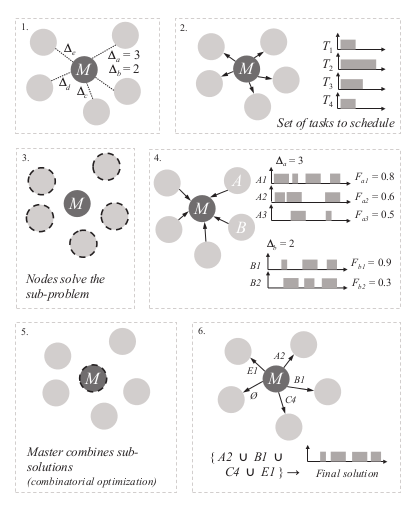
\includegraphics[scale=0.5]{Figures/LGsteps.png} 
\caption{Local-Global policy steps (as extracted from \cite{Araguz15})}
\label{LGsteps}
\end{figure}

To make possible the re-composition of the initial problem and to enable the master to find out the optimal combination taking into account as much information of the \emph{quality} of each local solution as possible, two parameters are defined: the figure of merit \emph{F} and the golden index $ \Delta $. The first of these parameters measures the goodness of each local solution, by combining a number of variables describing it. The second one is the number of possible solutions that each \emph{Local} entity can report to the global layer, and is meant to solve the possibly high heterogeneity in the system: nodes possessing higher processing capabilities will obtain a higher $ \Delta $ than those with lower computational resources.

Having described the basics of the Local-Global algorithm we will now specify the procedure it follows in six steps (see also Fig. \ref{LGsteps}):

\begin{enumerate}
\item \textbf{Characterization.} The $ \Delta $ value for each satellite is assigned, after considering its computing capabilities.
\item \textbf{Task delivery.} Master node selects the time window (duration of the schedule to be produced by the scheduloing algorithm) and discard tasks not fitting within it. After this, it sends to every \emph{Local} entity the set of tasks, so that they can begin to compute sub-solutions.
\item \textbf{Local evaluation.} Local entities' task planners produce as many solutions as its $ \Delta_i $ value, attaching each sub-solution an \emph{F} value.
\item \textbf{Submission of solutions.} Each satellite provides the set of at most $ \Delta_i $ solutions, sending for each one the list of tasks included in that schedule solution and its figure of merit \emph{F}.
\item \textbf{Global selection and combination.} The master triggers a combinatorial optimization process that selects at most one sub-solution per satellite in order to maximize the aggregated \emph{F} value, which is not necessarily the sum of the single \emph{F} values.
\item \textbf{Distribution of solution.} The master answer each \emph{Local} entity with the identity of its selected sub-solution, if any.

In section \ref{LGimplementation} we will focus on the implementation that has been developed in this Bachelor Thesis, specifying the \emph{Local} entity task planner characteristics and the optimization algorithm used in the global layer.
\end{enumerate}